\documentclass[a4paper,11pt,twoside]{scrartcl}
\usepackage[T1]{fontenc}
\usepackage[utf8]{inputenc}
\usepackage{ngerman, eucal, mathrsfs, amsfonts, bbm, amsmath, amssymb, stmaryrd, array, xcolor,graphicx, float, wrapfig}
\usepackage{epstopdf}
\usepackage{listings}
\usepackage[official]{eurosym}
\DeclareUnicodeCharacter{20AC}{\EUR{}}


\definecolor{middlegray}{rgb}{0.5,0.5,0.5}
\definecolor{lightgray}{rgb}{0.8,0.8,0.8}
\definecolor{orange}{rgb}{0.8,0.3,0.3}
\definecolor{yac}{rgb}{0.6,0.6,0.1}
\definecolor{green}{rgb}{0,.5,0}

\lstdefinestyle{c}{
	keywordstyle=\bfseries\ttfamily\color{blue},
	stringstyle=\color{orange}\ttfamily,
	commentstyle=\color{green}\ttfamily,
	emph={@Override, while, forall, if}, 
	emphstyle=\color{green}\texttt,
	emph={[2]List, Queue},
	emphstyle={[2]\color{yac}\texttt},
}
\lstset{
	basicstyle=\ttfamily,
	showstringspaces=false,
	flexiblecolumns=true,
	tabsize=2,
	numbers=left,
	numberstyle=\tiny,
	numberblanklines=false,
	stepnumber=1,
	numbersep=10pt,
	xleftmargin=15pt,
	breaklines=true,
	inputencoding=utf8
}

\lstdefinestyle{java}{
	language = java,
	emph={@Override}, 
	emphstyle=\color{teal}\texttt,
	emph={[2]Node,T,Comparable,AbstractNode,System, Thread,Random, Tree, Integer, Math, String, InterruptedException, Map, Entry, Point, TreeMap, PrintWriter, Scanner, FileReader, FileInputStream, FileNotFoundException, InputStreamReader, UnsupportedEncodingException, DecimalFormat, ArrayList, HashSet, LinkedList, IOException, HashMap, MapTest, MyHashMap, Puzzle, MyQueue, StringBuilder, NoSuchElementException, List, Queue, Vector, Tuple,Search, IllegalArgumentException, UnionFind, AbstractUnionFind, SpanningTree, Collections, WeightedEdge},
	emphstyle={[2]\color{yac}\texttt},
	texcl=true,
	keywordstyle=\color{blue}\ttfamily,
	stringstyle=\color{red}\ttfamily,
	commentstyle=\color{green}\ttfamily
}

\lstset{literate=
	{á}{{\'a}}1 {é}{{\'e}}1 {í}{{\'i}}1 {ó}{{\'o}}1 {ú}{{\'u}}1
	{Á}{{\'A}}1 {É}{{\'E}}1 {Í}{{\'I}}1 {Ó}{{\'O}}1 {Ú}{{\'U}}1
	{à}{{\`a}}1 {è}{{\`e}}1 {ì}{{\`i}}1 {ò}{{\`o}}1 {ù}{{\`u}}1
	{À}{{\`A}}1 {È}{{\'E}}1 {Ì}{{\`I}}1 {Ò}{{\`O}}1 {Ù}{{\`U}}1
	{ä}{{\"a}}1 {ë}{{\"e}}1 {ï}{{\"i}}1 {ö}{{\"o}}1 {ü}{{\"u}}1
	{Ä}{{\"A}}1 {Ë}{{\"E}}1 {Ï}{{\"I}}1 {Ö}{{\"O}}1 {Ü}{{\"U}}1
	{â}{{\^a}}1 {ê}{{\^e}}1 {î}{{\^i}}1 {ô}{{\^o}}1 {û}{{\^u}}1
	{Â}{{\^A}}1 {Ê}{{\^E}}1 {Î}{{\^I}}1 {Ô}{{\^O}}1 {Û}{{\^U}}1
	{œ}{{\oe}}1 {Œ}{{\OE}}1 {æ}{{\ae}}1 {Æ}{{\AE}}1 {ß}{{\ss}}1
	{ű}{{\H{u}}}1 {Ű}{{\H{U}}}1 {ő}{{\H{o}}}1 {Ő}{{\H{O}}}1
	{ç}{{\c c}}1 {Ç}{{\c C}}1 {ø}{{\o}}1 {å}{{\r a}}1 {Å}{{\r A}}1
	{€}{{\EUR}}1 {£}{{\pounds}}1
}
\usepackage{geometry}
\geometry{left=25mm, right=15mm, bottom=25mm}
\setlength{\parindent}{0em} 
\setlength{\headheight}{0em} 
\usepackage{eucal} %Matheschriften http://www.maths.usyd.edu.au/u/SMS/texdoc/euscript.pdf
\usepackage{mathrsfs} %schriften
\usepackage{amsfonts} %schriften https://www.ctan.org/pkg/amsfonts?lang=de
\usepackage{bbm} %Schriften http://mirrors.ctan.org/macros/latex/contrib/bbm/bbm.pdf
\usepackage{amsmath} %Mathezeug https://www.ctan.org/pkg/amsmath
\usepackage{amssymb} %Macros für Symbole https://www.ctan.org/pkg/amsfonts
\usepackage{stmaryrd} %Mehr Symbole ftp://ftp.rrzn.uni-hannover.de/pub/mirror/tex-archive/fonts/stmaryrd/stmaryrd.pdf

\newcommand{\grad}{\text{grad}}
\makeatletter
\g@addto@macro\bfseries{\boldmath} %Fette Mathe Symbole in Überschriften
\makeatother

\title{Datenstrukturen und effiziente Algorithmen\\ Blatt 12}
\author{Markus Vieth, David Klopp, Christian Stricker}
\date{\today}



\begin{document}

\maketitle
\cleardoublepage
\pagestyle{myheadings}
\markboth{Markus Vieth,  David Klopp, Christian Stricker}{Markus Vieth, David Klopp, Christian Stricker}

\section*{Aufgabe 1}
\subsection*{a)} 
Definiere zwei Farben (hier rot und blau)\\
Wähle einen beliebigen Knoten als ''CurrentVertex'' und setze ihn auf blau.\\

\begin{lstlisting}
Wiederhole {
	Füge alle Nachbarknoten in eine Warteschlange.
	Falls CurrentVertex blau und mindestens einer der Nachbarknoten auch blau {
		Rückgabe: FALSE
	} ansonsten {
		setze alle Nachbarknoten auf rot
	}
	
	Falls CurrentVertex rot und mindestens einer der Nachbarknoten auch rot {
		Rückgabe: FALSE
	} ansonsten {
		setze alle Nachbarknoten auf blau
	}
	Wähle den nächsten Knoten aus der Warteschlange als CurrentVertex
}

Falls die Liste leer ist {
	Rückgabe: TRUE
}
\end{lstlisting}
\subsection*{b)}
\subsubsection*{BipartiterGraph.java}
\lstinputlisting[style=java,basicstyle=\scriptsize\ttfamily]{Code/BipartiterGraph.java}
\section*{Aufgabe 2}


\section*{Aufgabe 3}
\subsection*{a)} 

\begin{center}
  \begin{tabular}{| c || c | c | c |}
    \hline
    Knoten & Input & Output & Differenz\\ \hline
    0 & 12     & 5 + 7 & 0 \\ \hline
    1 & 5       & 5       & 0 \\ \hline
    2 &  9      & 6 + 3 & 0 \\ \hline
    3 & 6 +7  & 13     & 0 \\ \hline
    4 & 0       & 0       & 0 \\ \hline
    5 & 0 + 3 & 3       & 0 \\ \hline
  \end{tabular}
\end{center}
Der Input ist niemals größer als die maximale Kapazität. Für alle Knoten bis auf $s$ und $t$ stimmt die Anzahl des Inputs mit der des Outputs  überein. Es handelt sich daher um einen gültigen Fluss.
\pagebreak
\subsection*{b)}
Nein, der eingezeichnete Fluss ist nicht maximal.
\begin{figure}[h]
\centering
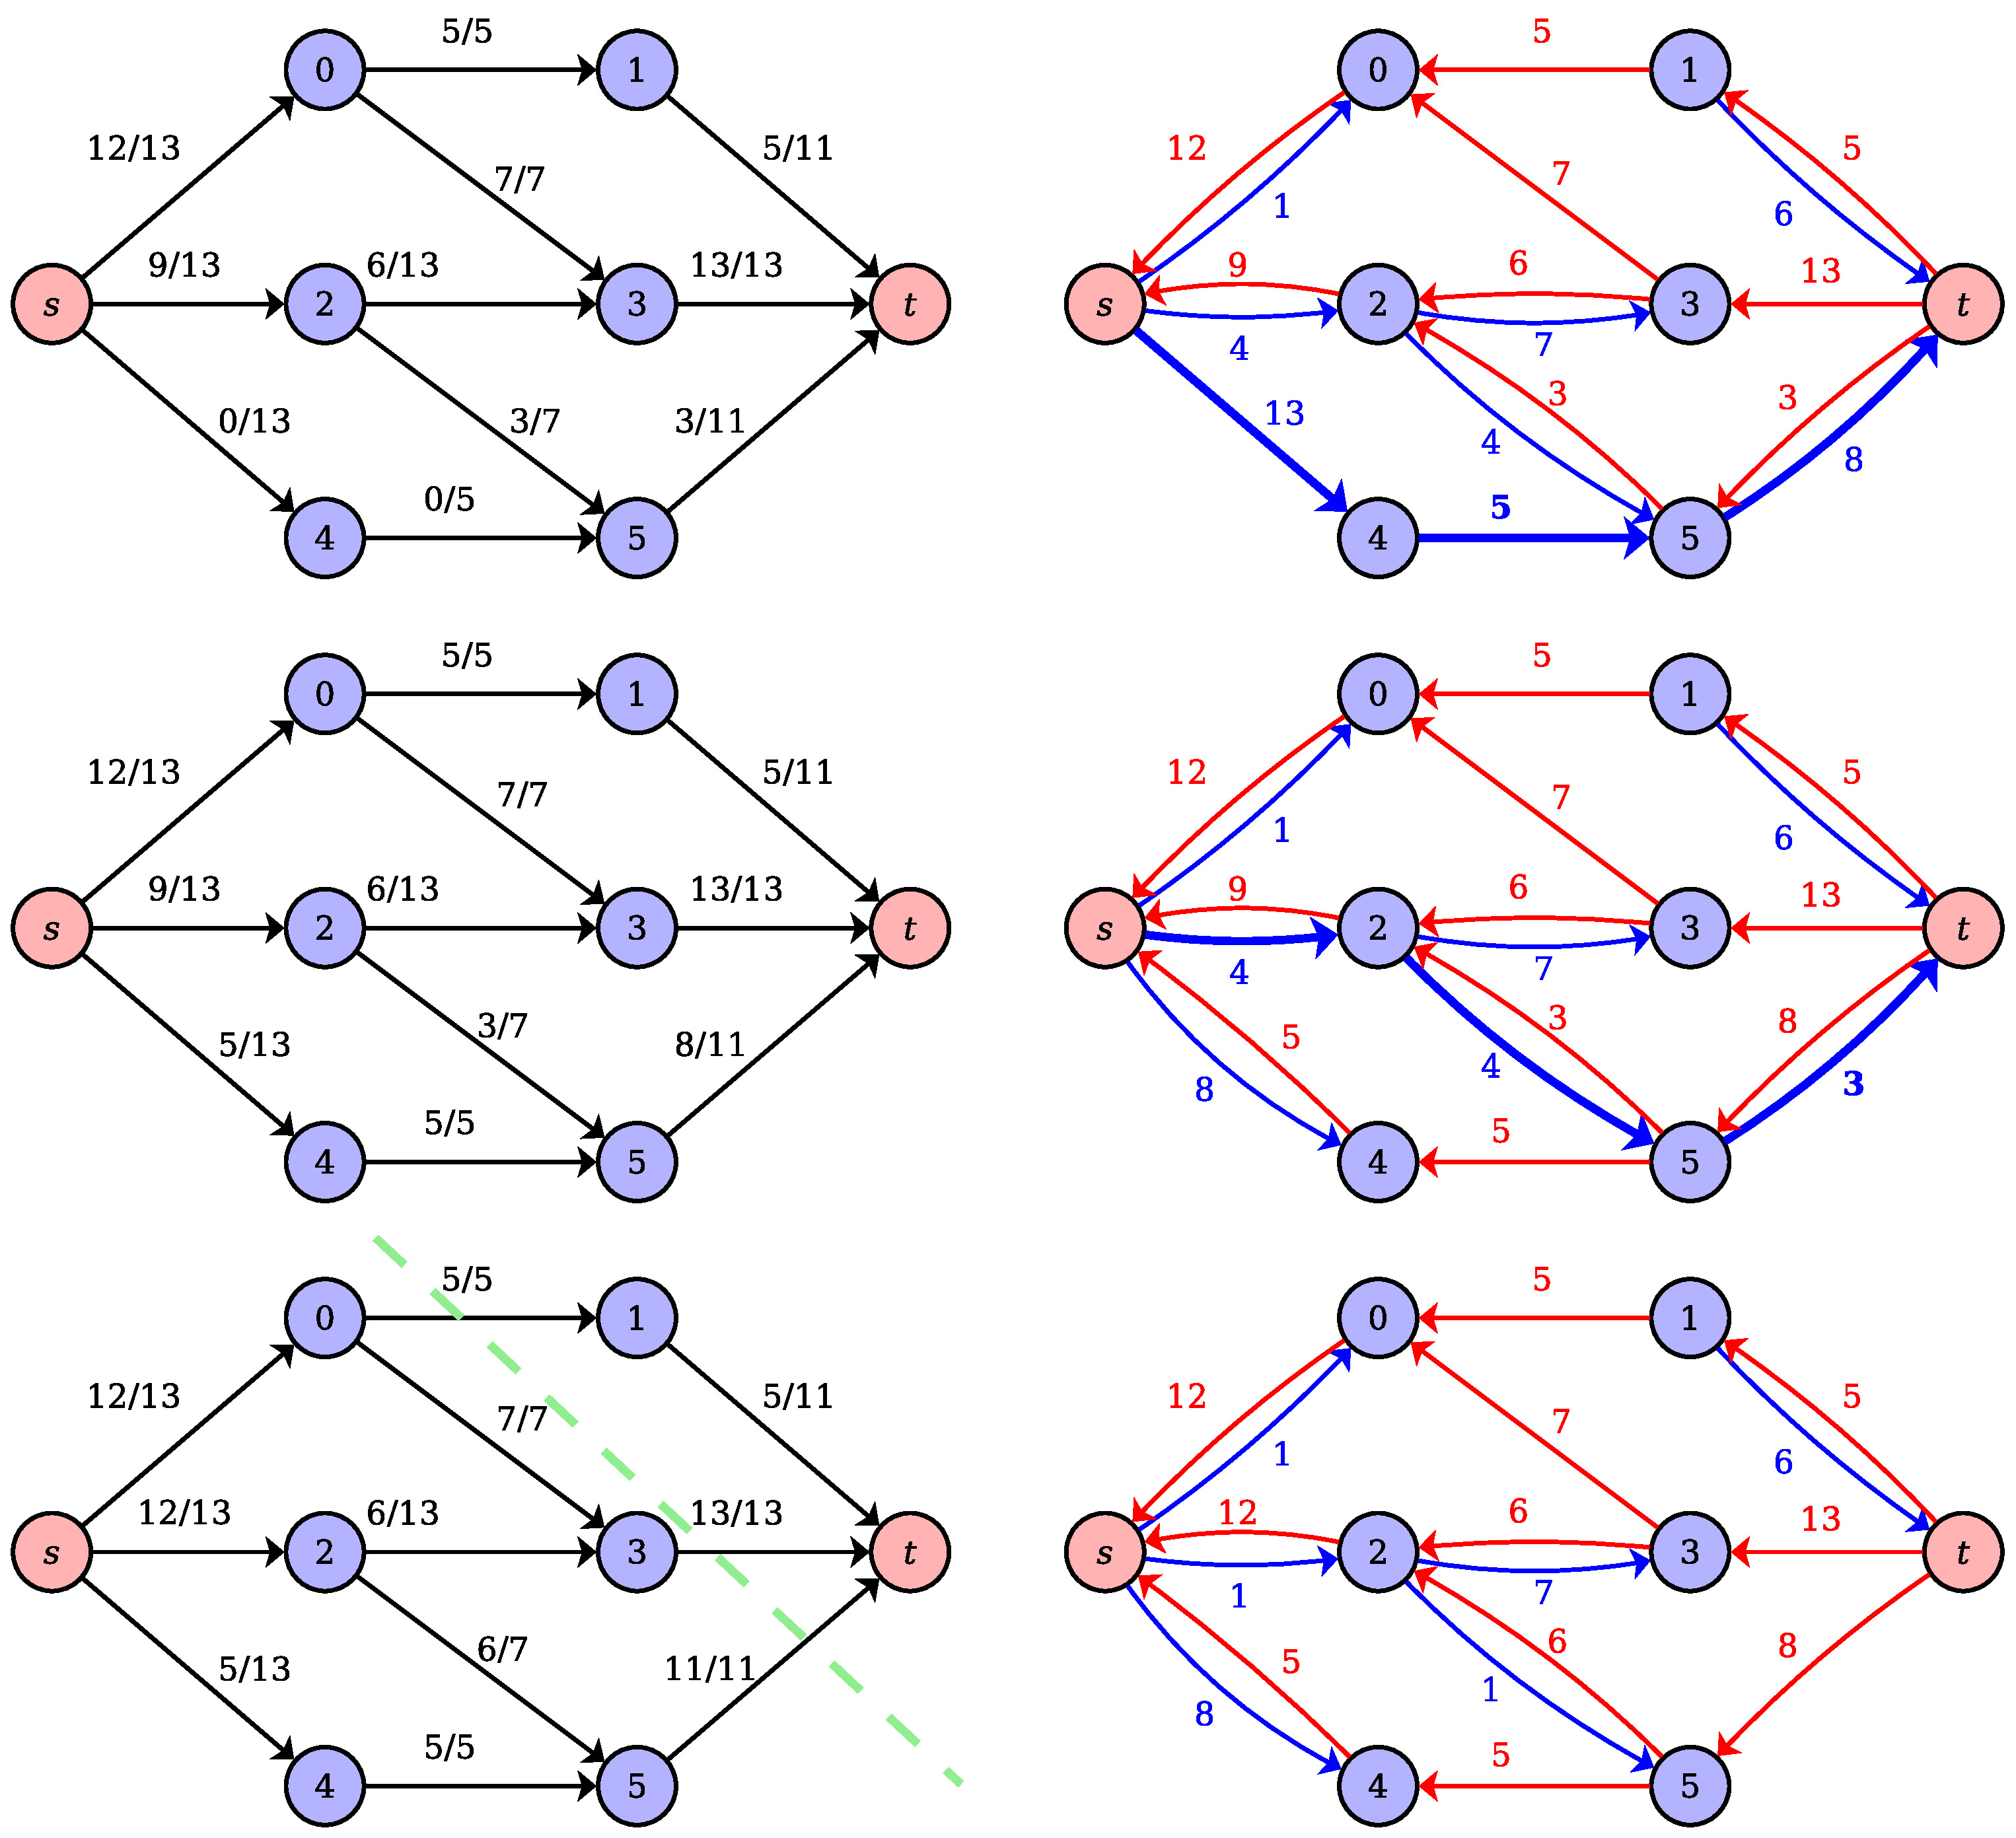
\includegraphics[width=\linewidth]{Grafik/Diagramm1}
\caption{Ford-Fulkerson}
\label{fig:Ford-Fulkerson}
\end{figure}
\subsection*{c)}
Siehe grüne, gestrichelte Linie. Der Schnitt geht durch die Kanten 0-1,3-t,5-t und entspricht dem maximalen Fluss (29).
\pagebreak
\subsection*{d)}

\begin{figure}[H]
	\centering
	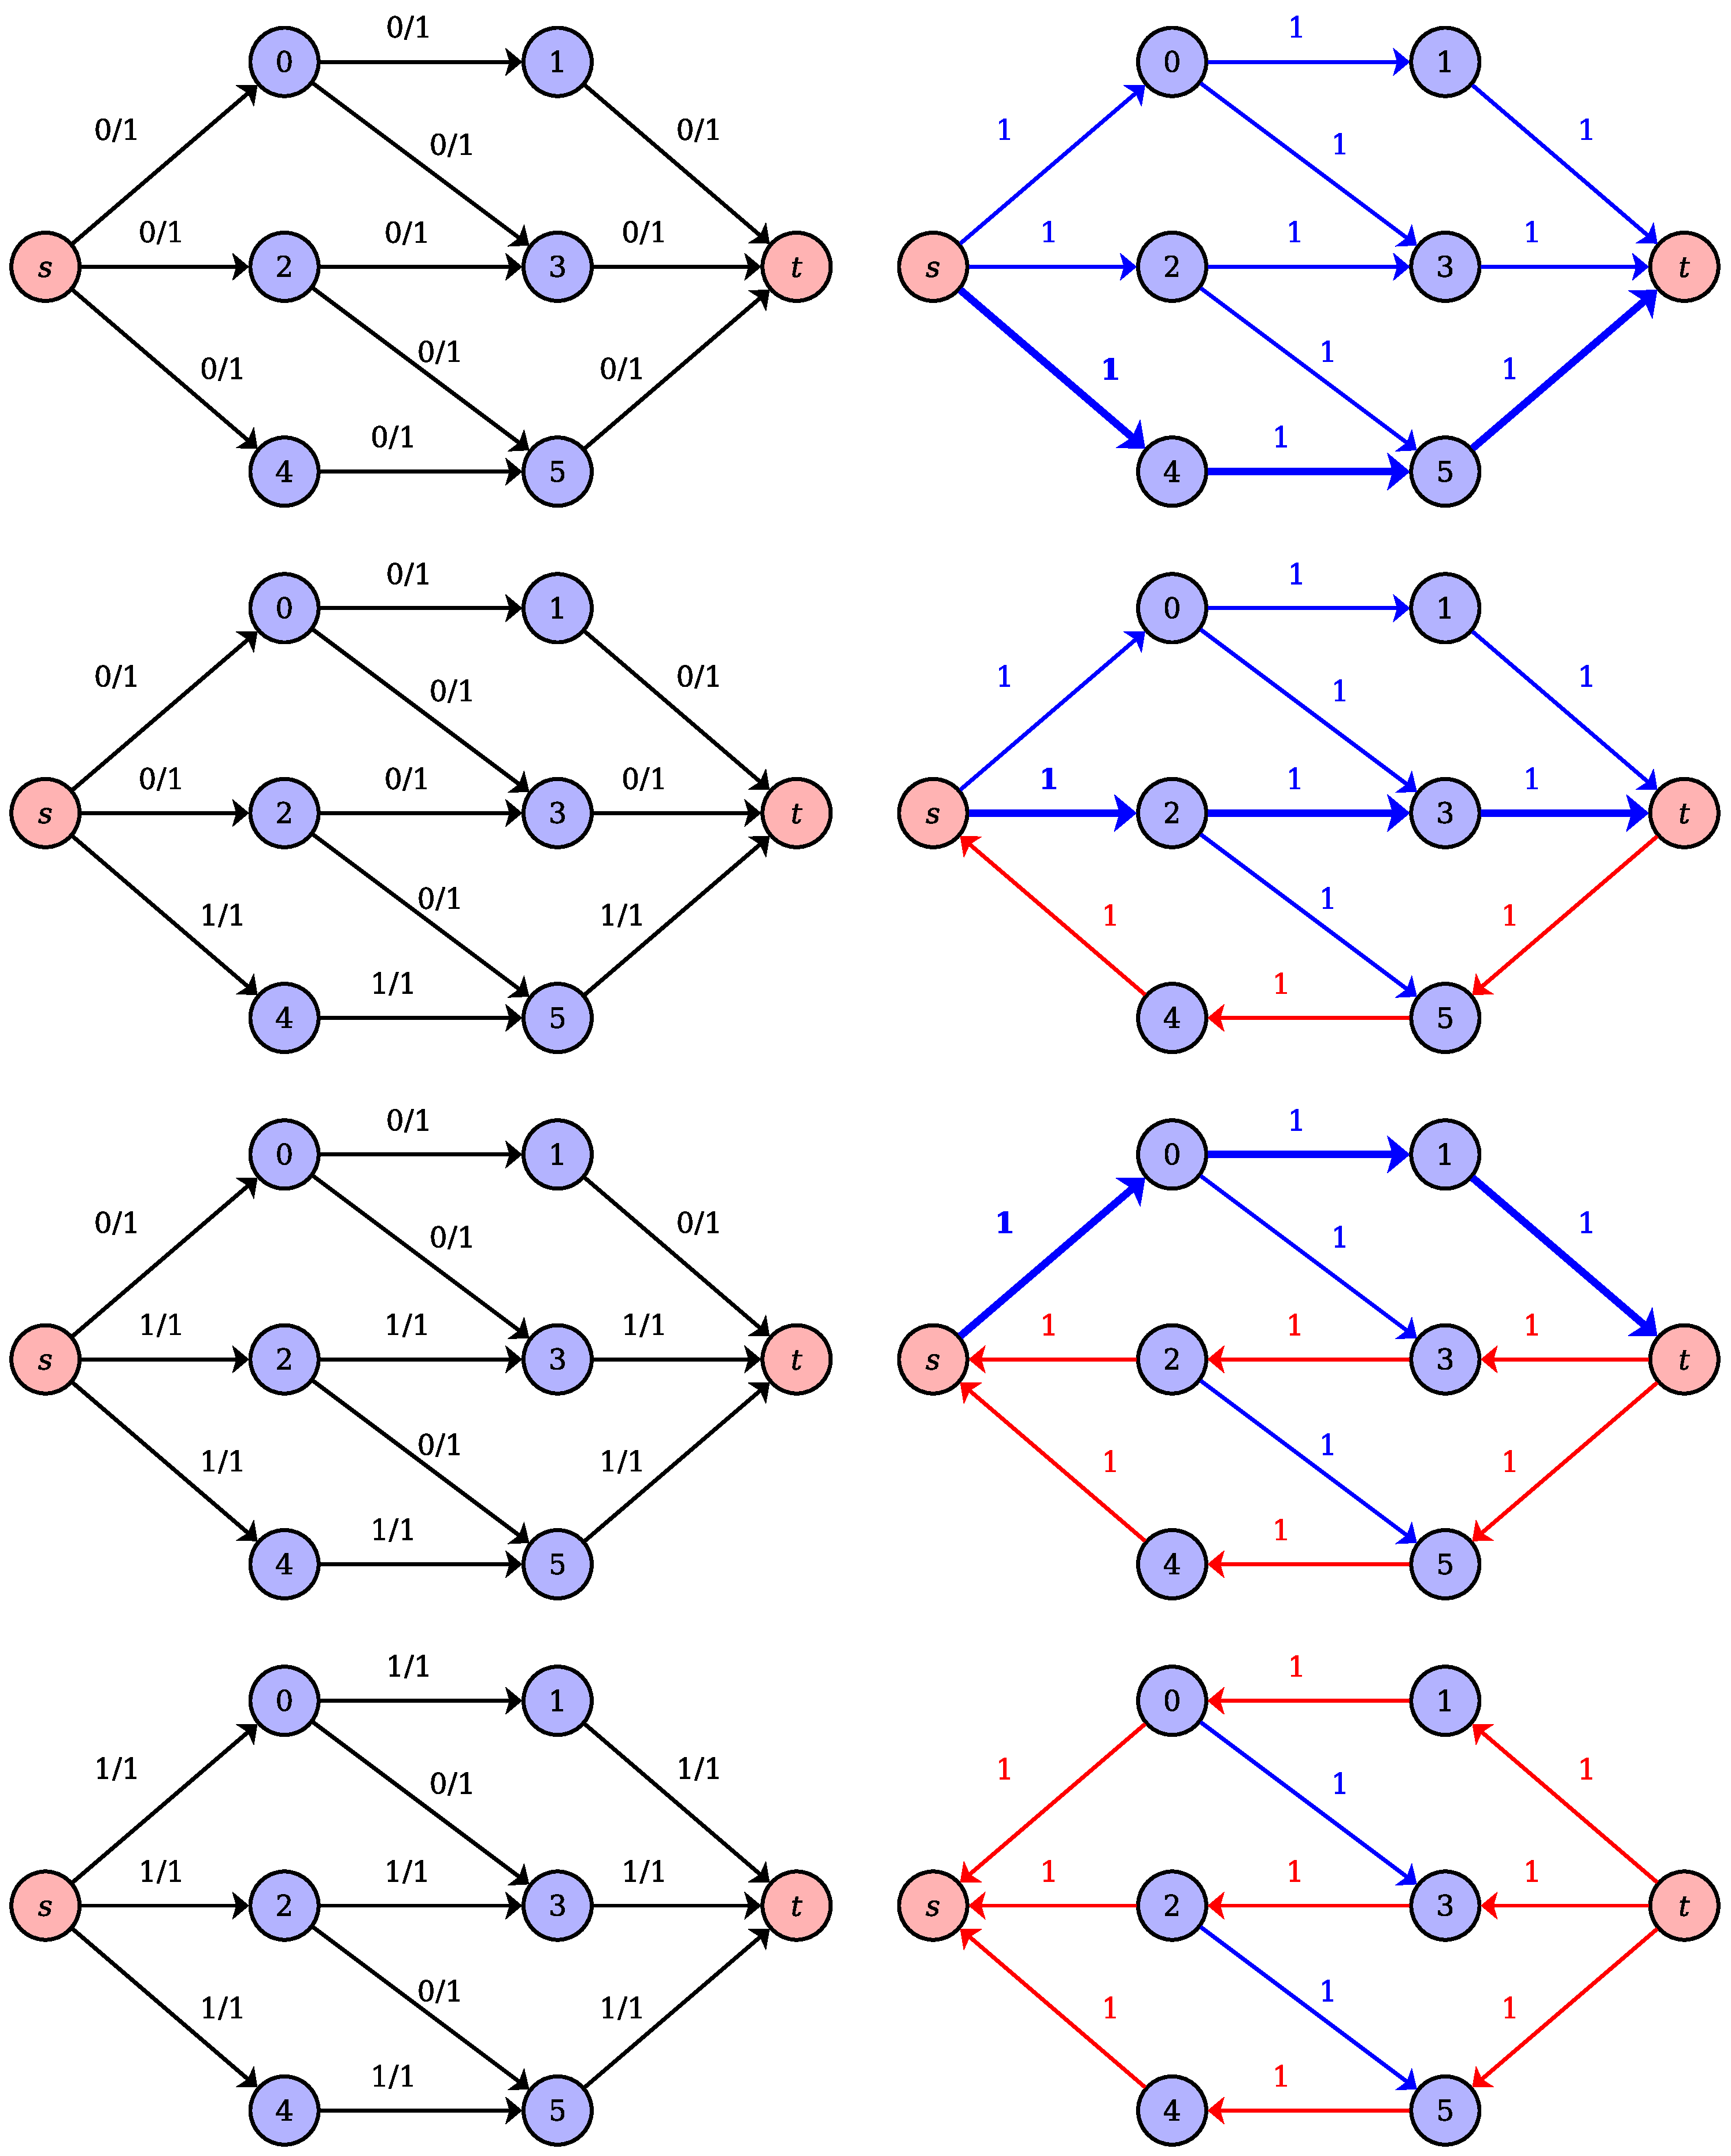
\includegraphics[width=0.75\linewidth]{Grafik/Diagramm2}
	\caption{Matching}
	\label{fig:Matching}
\end{figure}
In diesem Fall handelt es sich um ein Matching Problem. Wir haben die beiden Partitionen $A:=\{0,2,4\}~~B:=\{1,3,5\}$. Die lässt sich durch folgende Feststellungen belegen:
\begin{itemize}
	\item Es gibt nur Pfade von $A$ nach $B$
	\item Es gibt keine Pfade innerhalb von $A$ oder $B$
	\item $s$ ist mit allen Knoten aus $A$ verbunden und zu $t$ führen nur Kanten aus $B$
\end{itemize}
Entfernt man die Knoten $s$ und $t$, sowie alle mit diesen verbunden Kanten, erhält man einen bipartiten Graphen. Entfernt man nun noch alle Kanten mit einem Durchfluss von $0$ und macht aus den gerichteten Kanten ungerichtete, hat man ein maximales Matching.
\subsection*{Zusatzaufgabe: ResidualGraph.java}
\lstinputlisting[style=java,basicstyle=\scriptsize\ttfamily]{Code/ResidualGraph.java}
%\clearpage
%$ $
%\clearpage
\subsection*{Zusatzaufgabe: ResidualGraph.java}
\lstinputlisting[style=java,basicstyle=\ttfamily\scriptsize]{Code/ResidualGraph.java}
\end{document}